\documentclass[%
%10pt,
%varwidth=false,
%crop=true,
border={0mm 0mm 0mm 0mm}]{standalone}
\usepackage[T1]{fontenc}
\usepackage[utf8]{inputenc}
\usepackage[auto]{microtype}
%\usepackage{cmbright}
\usepackage{arev}
\usepackage{amsmath, amssymb, amsfonts, icomma}
\usepackage[version=4]{mhchem}
\usepackage{tikz}
\usetikzlibrary{positioning}
\usepackage{chemplants-tub}
\usepackage{xcolor}
%define stream tip, default is stealth
\setchpstreamtip{latex}
\setchpmainstreamthickness{thick}
%\setchpunitthickness{very thick}

\pgfdeclarelayer{bg}    % declare background layer
\pgfsetlayers{bg,main}  % set the order of the layers (main is the standard layer)

\definecolor{signalgruen}{RGB}{49,127,67}    % RAL 6032 Wasser
\definecolor{signalrot}{RGB}{155,36,35}      % RAL 3001 Dampf
\definecolor{signalgrau}{RGB}{150,153,146}   % RAL 7004 Luft
\definecolor{signalgelb}{RGB}{229,190,001}   % RAL 1003 brennbare und nicht brennbare Gase
\definecolor{signalorange}{RGB}{208,93,40}   % RAL 2010 Säuren
\definecolor{signalviolett}{RGB}{132,76,130} % RAL 4008 Laugen
\definecolor{signalbraun}{RGB}{121,77,62}    % RAL 8002 brennbare und nicht brennbare Flüssigkeiten
\definecolor{signalblau}{RGB}{30,45,110}     % RAL 5005 Sauerstoff
\definecolor{darkgreen}{RGB}{0,100,0} 

% TABLEAU-10
\definecolor{Tab10-A}{RGB}{78, 121, 167}
\definecolor{Tab10-B}{RGB}{242, 142, 43}
\definecolor{Tab10-C}{RGB}{225, 87, 89}
\definecolor{Tab10-D}{RGB}{118, 183, 178}
\definecolor{Tab10-E}{RGB}{89, 161, 79}
\definecolor{Tab10-F}{RGB}{237, 201, 72}
\definecolor{Tab10-G}{RGB}{176, 122, 161}
\definecolor{Tab10-H}{RGB}{255, 157, 167}
\definecolor{Tab10-I}{RGB}{156, 117, 95}
\definecolor{Tab10-J}{RGB}{186, 176, 172}

\begin{document}
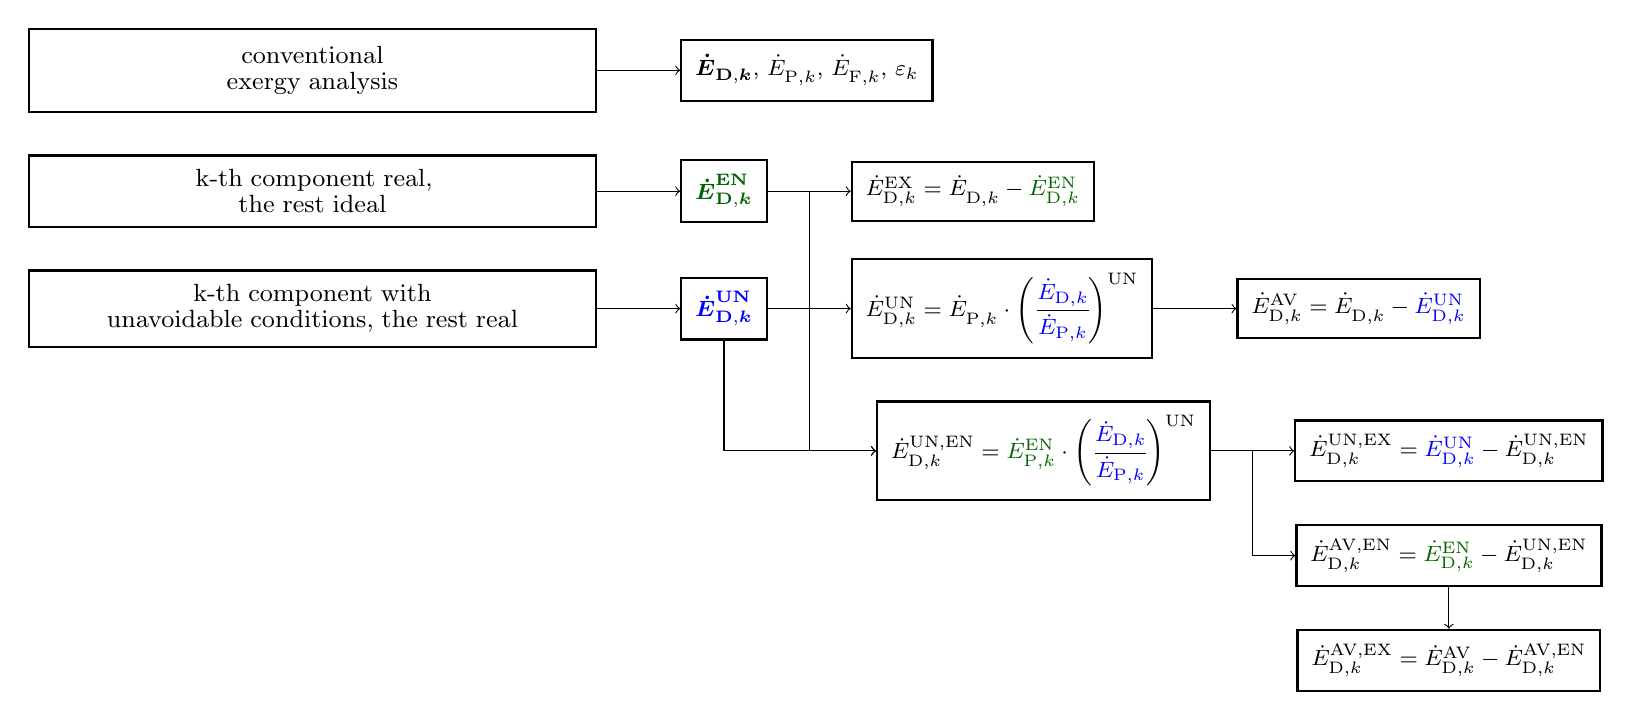
\begin{tikzpicture}[font=\footnotesize] 
%


% CONVENTIONAL EXERGY ANALYSIS
\node [rectangle, draw=black, minimum width=200pt, minimum height=30pt, text width=195pt, thick, inner sep=5pt, align=center] (conv) {\small conventional \\ exergy analysis};
% ED_k
\node [rectangle, draw=black, minimum height=22pt, thick, inner sep=5pt, align=center, right=30pt of conv] (ED) {$\boldsymbol{\dot{E}}_{\mathbf{D},\boldsymbol{k}}^{}$, $\dot{E}_{\text{P},k}^{}$, $\dot{E}_{\text{F},k}^{}$, $\varepsilon_k$};

% ENDOGENOUS
\node [rectangle, draw=black, minimum width=200pt, text width=195pt, thick, inner sep=5pt, align=center, below=15pt of conv] (endo) {\small k-th component real, \\ the rest ideal};
% EN
\node [rectangle, draw=black, thick, inner sep=5pt, align=center, right=30pt of endo] (EN) {\textcolor{darkgreen}{$\boldsymbol{\dot{E}}_{\mathbf{D},\boldsymbol{k}}^{\mathbf{EN}}$}};
% EX
\node [rectangle, draw=black, thick, inner sep=5pt, align=center, right=30pt of EN] (EX) {$\dot{E}_{\text{D},k}^\text{EX}=\dot{E}_{\text{D},k}^{}-\textcolor{darkgreen}{\dot{E}_{\text{D},k}^\text{EN}}$};

% UNAVOIDABLE
\node [rectangle, draw=black, minimum width=200pt, text width=195pt, thick, inner sep=5pt, align=center, below=15pt of endo] (unavoid) {\small k-th component with \\ unavoidable conditions, the rest real};
% UN uncorrected
\node [rectangle, draw=black, thick, inner sep=5pt, align=center, right=30pt of unavoid] (UN) {\textcolor{blue}{$\boldsymbol{\dot{E}}_{\mathbf{D},\boldsymbol{k}}^{\mathbf{UN}}$}};
% UN corrected
\node [rectangle, draw=black, thick, inner sep=5pt, align=center, right=30pt of UN] (UN_corrected) {$\dot{E}_{\text{D},k}^{\text{UN}} = \dot{E}_{\text{P},k}^{} \cdot \left( \cfrac{\textcolor{blue}{\dot{E}_{\text{D},k}}}{\textcolor{blue}{\dot{E}_{\text{P},k}}} \right)^\text{UN}$};
% AV
\node [rectangle, draw=black, thick, inner sep=5pt, align=center, right=30pt of UN_corrected] (AV) {$\dot{E}_{\text{D},k}^{\text{AV}} = \dot{E}_{\text{D},k}^{} - \textcolor{blue}{\dot{E}_{\text{D},k}^{\text{UN}}}$};

% UNAVOIDABLE-ENDOGENOUS
\node [rectangle, draw=black, thick, inner sep=5pt, align=center, below=15pt of UN_corrected, shift={(15pt, 0)}] (UN_EN) {$\dot{E}_{\text{D},k}^{\text{UN,EN}} = \textcolor{darkgreen}{\dot{E}_{\text{P},k}^\text{EN}}\cdot \left( \cfrac{\textcolor{blue}{\dot{E}_{\text{D},k}}}{\textcolor{blue}{\dot{E}_{\text{P},k}}} \right)^\text{UN}$};
% UNAVOIDABLE-EXOGENOUS
\node [rectangle, draw=black, thick, inner sep=5pt, align=center, right=30pt of UN_EN] (UN_EX) {$\dot{E}_{\text{D},k}^{\text{UN,EX}} = \textcolor{blue}{\dot{E}_{\text{D},k}^{\text{UN}}} - \dot{E}_{\text{D},k}^{\text{UN,EN}}$};
% AVOIDABLE-ENDOGENOUS
\node [rectangle, draw=black, thick, inner sep=5pt, align=center, below=15pt of UN_EX] (AV_EN) {$\dot{E}_{\text{D},k}^{\text{AV,EN}} = \textcolor{darkgreen}{\dot{E}_{\text{D},k}^\text{EN}} - \dot{E}_{\text{D},k}^{\text{UN,EN}}$};
% AVOIDABLE-EXOGENOUS
\node [rectangle, draw=black, thick, inner sep=5pt, align=center, below=15pt of AV_EN] (AV_EX) {$\dot{E}_{\text{D},k}^{\text{AV,EX}} = \dot{E}_{\text{D},k}^\text{AV} - \dot{E}_{\text{D},k}^{\text{AV,EN}}$};



\draw [->] (conv.east) -- (ED.west);
\draw [->] (endo.east) -- (EN.west);
\draw [->] (EN.east) -- (EX.west);
\draw [->] (unavoid.east) -- (UN.west);
\draw [->] (UN.east) -- (UN_corrected.west);
\draw [->] (UN_corrected.east) -- (AV.west);
\draw [->] (EN.east) -- ++(15pt,0) |- (UN_EN.west);
\draw [->] (UN.south) -- ++(0,0) |- (UN_EN.west);
\draw [->] (UN_EN.east) -- (UN_EX.west);
\draw [->] (UN_EN.east) -- ++(15pt,0) |- (AV_EN.west);
\draw [->] (AV_EN.south) -- (AV_EX.north);
\end{tikzpicture}
\end{document}